\newpage
%\section{Introduction}
\chapter{Introduction}
\label{sec:introduction}
\section{Motivation}

This master thesis is part of the NTNU SmallSat \cite{SmallSat_project_description} project. The projects mission is to use hyperspectral imaging to observe ocean color in the ocean and the coast of Norway. The payload of the satellite will be a 1/3 U push-broom type hyperspectral imager, dedicated to take images of a $30x50 km^2$ area. In regular Red Green Blue(RGB) imaging each of the image pixels is made up of three frequency components that represent the intensities in red, green and blue frequencies respectively. Such a component is referred to as a band. In hyperspectral imaging, a pixel will typically consists of hundreds to thousands of bands, providing more information than regular images. This information can be used for a lot of different purposes. It can for example be used to detect different materials in an area, by using spectral signatures of materials as identifiers. This is shown in Figure \ref{fig:HSI_concept}.\\

\begin{figure}[H]
\centering
   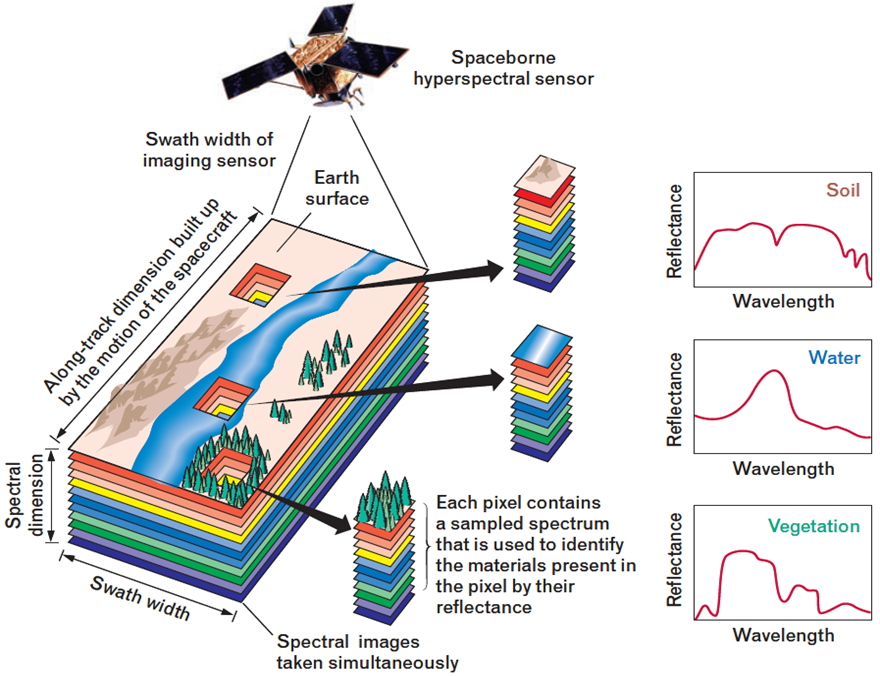
\includegraphics[scale=0.4]{images/Imaging-Spectroscopy-Concept.png}
  \caption{ Functional concept of HSI.\cite{HSI_concept} } 
  \label{fig:HSI_concept}
\end{figure}


\\

NTNU SmallSat aims to use this information to detect algae blooms, phytoplankton, oil spills, microplastic and possibly other irregularities or \textit{anomalies} in the ocean. Detection of harmful algae blooms (HABs) is particularly interesting for the salmon farms located along the coast of Norway, as such blooms can be toxic, even deadly, for the salmon. Algaes were most likely the cause of death for 38 000 salmons in southern Troms in September of 2017 \cite{laksedeath}. An image of such a bloom can be seen in Figure \ref{fig:algae_bloom_troms}. Increasing ocean temperatures as a consequence of global warming may lead to more frequent and intense HABs \cite{climate_change_algae_blooms}. 
%With the increasing rise in sea temperatures and the issues faced with global warming this is an even 
% HSI  = hyperspectral imager or imaging?
\\

\begin{figure}[H]
\centering
   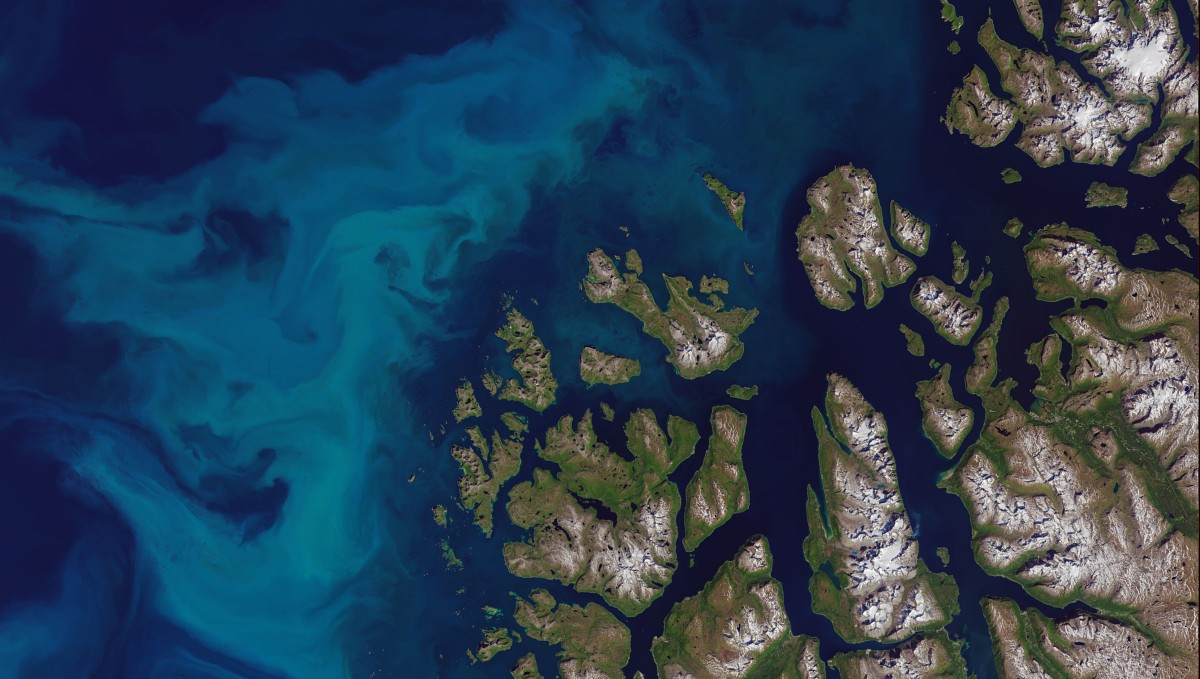
\includegraphics[scale=0.3]{images/algaes/algaes_northern_troms.jpg}
  \caption{ Image of an algae bloom along the coast of Troms in Norway \cite{laksedeath}. Foto by NASA EARTH OBSERVATORY. } 
  \label{fig:algae_bloom_troms}
\end{figure}
\\

Algaes will have spectral signature that is different to the background, which will be ocean water or land. Algaes may therefore be considered \textit{anomalies}. An anomaly in the context of HSI is a spectral pixel vector that have significant spectral differences from its surrounding background pixels \cite{yang2015dual}.  
\\

Anomaly detection may help combat and monitor the challenges faced globally as a consequence of global warming and human pollution. One of these challenges is the vast amount of micro-plastic(plastic particles smaller than $5mm$) in the worlds oceans. Anomaly detection may be used to detect spots of ocean water having higher density of micro-plastic than the surrounding ocean water, if such spots exists.       \\



%%It does not say anything about 54 seconds in that description...
According to \cite{SmallSat_project_description} the time requirements for actual detection of pushbroom scanning and HSI operations is 54 seconds. The goal of the Anomaly detector(AD) is to be able to operate in near-realtime or realtime, using at most 54 seconds. 

\\
%Say something about the AD being part of a larger processing pipeline? Power, area, resources, as this is a solar powered device?





\newpage
\subsection{Master thesis overview}
The following chapters in this project report delve into the implementation of an AD on a Xilinx Virtex-7 FPGA. The AD is made for the Smallsat project \cite{SmallSat_project_description}. \\  

Chapter \ref{sec:theory} is the Theory section.  Algorithms considered used for anomaly detection are described in this chapter. This include the Reed-Xiaoli algorithm, the Local Reed-Xialoi algorithm, the Adaptive Causal algorithm and a proposed AD algorithm by the author, called the Adaptive Local Reed-Xiaoli algorithm. Theory about inverse computation is also found in this chapter.   \\


Chapter \ref{chapter:review_anomaly_detectors} contains the review of the considered ADs presented in chapter \ref{sec:theory}. In this section tests of the different anomaly-detectors has been done in MATLAB on synthetic images and on real image data from the Cuprite scene.\\  

In Chapter \ref{sec:implementation} the hardware implementation of the AD is described. The architecture is presented, along with different design considerations. 

\\

Chapter \ref{sec:results} is the Results section. This section contains synthesis results, simulation results and results from testing on HW.
\\

Chapter \ref{sec:Discussion} is the Discussion section. 
\\

Chapter \ref{sec:conclusion} is the Conclusion section. The most important results are presented here.  Future work that can be done is mentioned.
\\




